% \documentclass[12pt,draftclsnofoot,peerreview,onecolumn]{IEEEtran}
\documentclass[12pt, draftclsnofoot, onecolumn]{IEEEtran}
% \documentclass[journal,comsoc, onecolumn, 12pt,draftclsnofoot]{IEEEtran} % ,]
% \documentclass[journal,comsoc]{IEEEtran}
\usepackage[T1]{fontenc}
% \usepackage{cite}
% \usepackage{amsfonts}
\usepackage{amssymb}
\usepackage{amsmath}
\usepackage{array}
\interdisplaylinepenalty=2500
\usepackage{filecontents}
\usepackage{url}
\usepackage{bm}
\usepackage[square,sort,comma,numbers]{natbib}
\usepackage{subfigure} 
% \usepackage{caption}
% \usepackage{subcaption}
\usepackage[colorlinks,
  linkcolor=black,
  anchorcolor=blue,
  citecolor=black
  ]{hyperref}
\ifCLASSINFOpdf
 \usepackage[pdftex]{graphicx}
\else
 \usepackage[dvips]{graphicx}
\fi

% \usepackage[GREY]{epspdfconversion}
% \usepackage{lineno}
% \linenumbers 

% correct bad hyphenation here
\hyphenation{op-tical net-works semi-conduc-tor}

\renewcommand{\citedash}{--}

\DeclareMathOperator*{\argmax}{arg\,max}

\begin{document}
%
% paper title
% can use linebreaks \\ within to get better formatting as desired

\title{Entropy Minimization Based Symbol Timing
\\and Carrier Frequency Recovery}
% \author{\IEEEauthorblockN{Xiao Liu and Jean-Fran\c{c}ois Bousquet }
% \IEEEauthorblockA{Electrical and Computer Engineering\\
% Dalhousie University\\
% Halifax, B3H 4R2, Canada\\
% Email: x.liu@dal.ca}}
\author{Xiao~Liu,~\IEEEmembership{Student Member,~IEEE,}
%         John~Doe,~\IEEEmembership{Fellow,~OSA,}
        and~Jean-Fran\c{c}ois~Bousquet,~\IEEEmembership{Member,~IEEE}% <-this % stops a space

\thanks{Manuscript received February, 2018; revised xxxx xx, 2018. This project was supported by the Atlantic Innovation Fund \#Project \#203162.}
\thanks{The authors are with the Department of Electrical and Computer Engineering, Dalhousie University, Halifax,
NS, B3J 1Z1, Canada (e-mail: \{x.liu, jbousquet\}@dal.ca).}% <-this % stops a space
% \thanks{J. Bousquet is with Dalhousie University.}% <-this % stops a space
}

% The paper headers
% \markboth{IEEE Transactions on Communications,~Vol.~xx, No.~x, xxxxxx~2017}
% {Shell \MakeLowercase{\textit{et al.}}: Entropy Minimization Based Symbol Timing and Carrier Frequency Recovery}

% make the title area
\maketitle


\begin{abstract}
This paper presents a new entropy minimization criterion for both symbol timing and carrier frequency recovery for  wireless receivers.
The synchronization is achieved by minimizing the entropy estimated from the eye diagram and the constellation diagram. 
A custom entropy estimation algorithm is proposed to accelerate the searching of quadratic R\'enyi entropy with a kernel function.
Several practical issues are addressed in implementing the entropy based synchronization algorithms.
% achieve fast estimation of the synchronization parameters.
% Also, an entropy minimization based synchronization implementation with reduced complexity is described and its 
Also, the performance of the proposed algorithm is evaluated in controlled conditions.
% , as well as with realistic measurement data acquired during an underwater communication sea trial.
It is shown that, as an alternative to maximum likelihood criterion, entropy minimization has great potential and offers certain advantages for synchronization in wireless communication, particularly with small excess bandwidth as well as in multipath channel conditions. 

\end{abstract}

% {\bf Keywords:} 
\begin{IEEEkeywords}
Entropy minimization, symbol timing, carrier frequency recovery, synchronization, multipath.
\end{IEEEkeywords}

\IEEEpeerreviewmaketitle

\section{Introduction}
\label{sec:intro}
\IEEEPARstart{I}{n} coherent wireless communications systems, ``synchronization'' is a key operation at the receiver.
It is usually realized between the matched filter and the equalizer.
The two main functions of the synchronizer are symbol timing and carrier recovery.
The purpose of symbol timing recovery is to recover the symbol clock from the modulated waveform, so that it can down sample the waveform with the correct symbol timing offset (STO).
Hence, at the output of a matched filter, the signal sampled at the ideal instant can have maximum signal to noise ratio (SNR) and no intersymbol interference~(ISI)~\cite{mengali1997synchronization}.
Also, in coherent communication systems, the down converter must have exactly the same frequency as the carrier of the signal to recover the information embedded in the phase modulation. 
However, in practice, the local oscillator frequency deviates from the input signal's carrier frequency. 
As such, the carrier frequency offset~(CFO) has to be compensated. 
In modern orthogonal frequency division multiplexing (OFDM) based systems, the CFO recovery is essential because the frequency offset results in loss of orthogonality between the OFDM carriers.
Moreover, in some applications, such as underwater acoustic communications, the channel may constantly change due to the time-variant environment or Doppler effect. 
Therefore a continuous estimation and compensation of the STO and CFO is essential to maintain the link reliability.

% \textbf{a summary of standard solutions }
Various synchronization algorithms have been described in the literature.
% They are generally characterized by their structures or the availability of training data.
While data-aided (DA) synchronization offers a superior performance, in this work, non-data-aided (NDA) algorithms are proposed to maintain a high spectral efficiency.
A feedforward timing correction architecture is described for fast convergence rate. 
% implemented in a feedforward architecture are preferred for fast convergence, high spectral efficiency transmission.  


% They can be either feedforward or feedback depending on their configurations.
% Also, the algorithms can also be categorized to data-aided (DA) or non-data-aided (NDA) according to the availability of training data. 
% The \textit{feedforward} structure directly extracts the timing tone or CFO  from the incoming signal.
% Whereas the \textit{feedback} structure uses a timing (or frequency) error detector to derive an error signal and feeds it back to recover the synchronization parameters.
% On the other hand, 


% is supervised, otherwise it is unsupervised.
% This categorization is also known as \textit{data-aided} (DA), \textit{decision-directed} (DD) and \textit{non-data-aided} (NDA) 

Most synchronization algorithms follow the maximum likelihood (ML) criterion or its approximation.
For example, the Oerder and Meyr (O\&M) algorithm~\cite{Oerder1988} is a magnitude-squared nonlinear spectral line method exploiting the cyclostationary properties of the modulated signal, 
and is one of the most commonly used NDA feedforward algorithm for symbol timing recovery.
It has been proven that this algorithm and its variants can be asymptotically interpreted as a ML estimator~\cite{YanWang2002,Lopez-Salcedo2006}.
Also, the NDA Gardner timing error detector~\cite{Gardner1986} and its DA counterpart, the zero-crossing detector~\cite{gardner1988demodulator} can be derived from the ML criterion~\cite{Oerder1987}.
For carrier recovery, the NDA feedforward CFO estimator proposed in~\cite{Wang2004} employs the fourth-order cyclostationary property, and still follows the ML criterion.
Also, various DA feedforward CFO estimation algorithms attempt to maximize the inner product between the  training sequence and the data samples.
In~\cite{Li2008,Amar2017},
% * <x.liu@dal.ca> 2018-02-06T17:15:31.656Z:
% 
% How to make multiple citations together?
% 
% ^.
the CFO in OFDM communication is estimated by minimizing a quadratic cost function.
All these methods can be treated as generalized ML estimators.
% The ML criterion assumes a Gaussian and linear system, two conditions that are not always satisfied in reality. 

% \textbf{What is scope of this paper }
% In this paper, we consider entropy minimizes (EM) as an alternative criterion for synchronization parameter estimation.
The primary contribution of this paper consists in the definition of a unified synchronization principle, the entropy minimization (EM) as an alternative to the ML criterion. 
Specifically, the entropy of the eye diagram is evaluated for symbol timing recovery, and the entropy of the constellation diagram is measured for carrier frequency recovery.
For both applications, the synchronization parameter that leads to a minimum entropy value is considered to be optimum.
% and the objective function based on this criterion is applied to both symbol timing and carrier frequency recovery.
% Like the ML criterion, it aims to optimize a unified objective function.
% The algorithms that will be applied in this work are NDA and implemented in a feedforward structure, but they can be extended to other configurations under the same criterion.
Note that it has been shown in~\cite{Pedzisz2006} that the CFO of phase-shift keying (PSK) modulated signals can be recovered by minimizing the entropy of the instantaneous phase probability density function (PDF).
% Also, it has been reported that the error entropy minimization algorithms can be applied for channel equalization \cite{Santamaria2002}. 
However, the CFO estimation in this work is applied to a broader type of modulation schemes, and to the authors' knowledge, the unified criterion for both symbol timing and carrier recovery has not been proposed before. 

Since Shannon's work~\cite{Shannon1948}, entropy is an important concept in information theory. 
However, it is rarely used in practice, because it is difficult to estimate directly from samples without a model~\cite{Bercher2000}.
Therefore, researchers are constantly developing express entropy estimation methods for their specific applications.
For example, in the study of physiological data, the simplified approximate entropy (ApEn)~\cite{Pincus1991}, and sample entropy (SampEn)~\cite{Richman2000} are used to estimate the complexity of the time series.
As a second contribution of this work, a custom entropy estimation algorithm is proposed to accelerate the searching,
where a kernel function is used to estimate the quadratic R\'enyi entropy.
% ~\cite{Santamaria2002,Huang2008}.

Many practical issues can be encountered when implementing EM based synchronization algorithms.
These issues include undesired local minima, insufficient oversampling rate and the vanishing of the gradient.
The third contribution of this work is a practical implementation that addresses these issues.

The final part of this work is the evaluation of the  algorithm performance in controlled conditions. 
% as well as in realistic underwater acoustic propagation conditions.  
The effect of various channel impairments, including noise and multipath, is analyzed on the system performance.  
The EM based algorithms are found to have improved performance when the signal has a small excess bandwidth, so that it allows to provide better spectral efficiency.
It is also demonstrated that ML based algorithms cannot achieve ideal synchronization in multipath channel propagation, while the EM criterion is a better choice in such conditions. 
% PMF not PDF
% Unlike these systems, this paper focuses on
%  \textbf{contributions}
% The contribution of this work is summarized as below.
% 1)~The entropy minimization (EM) criterion is studied for symbol timing and carrier frequency recovery.
% 2)~An ad-hoc entropy estimation algorithm is proposed for fast parameter estimation.
% 3)~The practical issues of EM based synchronization algorithms is discussed. 



This paper is organized as follows.
In Section~\ref{sec:entropy},
an entropy minimization criterion for synchronization is introduced. 
In Section~\ref{sec:cust_entp}, a customized fast entropy estimation algorithm is described. 
The algorithm implementation issues are addressed in Section~\ref{sec:imple}.
In Section~\ref{sec:perfo}, the performance of the algorithms is evaluated in controlled conditions.
% , and the algorithm is also applied to realistic data.  
Finally, conclusions are drawn in Section~\ref{sec:conc}.
% \clearpage
%%%%%%%%%%%%%%%%%%%%%%%%%%%%%%%%%%%%%%%%%%%%%%%%%%

\section{Entropy Minimization Based Synchronization}
\label{sec:entropy}
In this section, the signal model adopted in this paper is presented in Section~\ref{sec:model}.
The standard ML criterion is briefly introduced in comparison to the EM criterion in Section~\ref{sec:versus}.
% we are going to use through this article.
% Then, the application of the EM criterion to symbol timing and carrier frequency recovery using the eye diagram and constellation diagram is explained.
Then, the application of the EM criterion to symbol timing using the eye diagram entropy is explained in Section~\ref{sec:eye_entp},
while the constellation diagram entropy used for carrier frequency recovery is explained in Section~\ref{sec:const_entp}.
% An ad-hoc entropy estimation algorithm is proposed in the last part of this section for fast synchronization parameter search.
\subsection{Signal Model }  
\label{sec:model}
% There are other forms of definitions or expressions of entropy that won't be detailed here.
% We will focus on how entropy can be applied in symbol timing and carrier frequency recovery.

In this work, it is assumed that the signal is transmitted using coherent modulation schemes with an alphabet size of \(M\), where \(M\) is usually a power of 2.
In the following discussion, quadrature phase shift keying (QPSK) modulation is used to validate the performance, but the application is not limited to low order modulation schemes.
The received binary information follows an independent identical distribution (i.i.d.).
The modulated data is pulse shaped to limit the bandwidth occupancy.
A standard pulse shaping filter is used at the transmitter, which is designed under the Nyquist criterion, 
such that there is no ISI at the ideal sampling instants.

% \begin{figure*}[ht]
% \centering
% 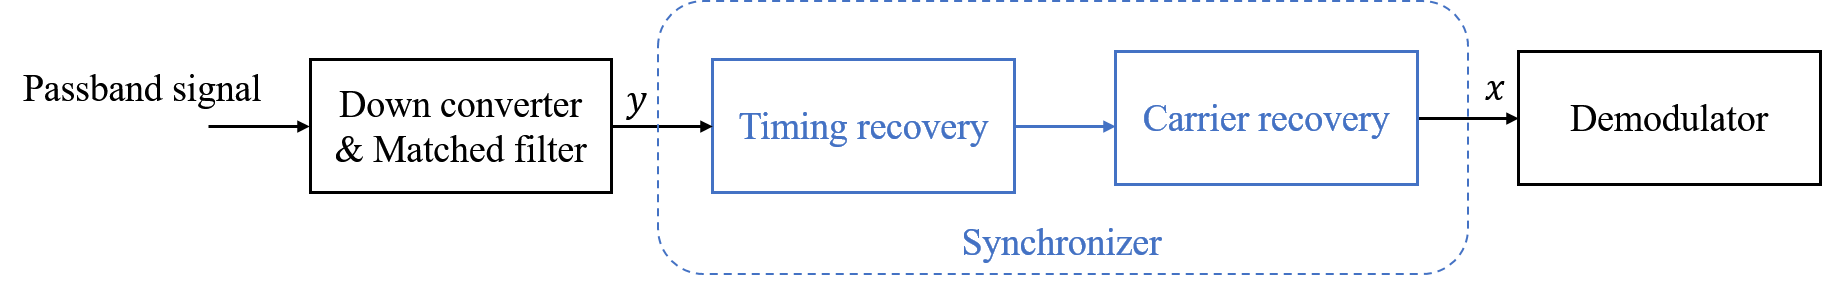
\includegraphics[width=5.5 in]{pic/sys_conf.png}
% \caption{Block diagram of the receiver configuration.}
% \label{fig:sysconf} 
% \end{figure*}

% Fig.~\ref{fig:sysconf} shows the block diagram of the receiver configuration.
The receiver configuration is given below.
The received passband signal goes through a down converter and a matched filter first.
% The matched filter is the same RRC filter used in pulse shaping, so the overall filter becomes a raised-cosine~(RC) filter. 
% The following block is the the synchronizer, which is used for both timing and carrier recovery. 
% The matched filter is the same RRC filter used in pulse shaping, so the overall filter becomes a raised-cosine~(RC) filter. 
Then, the timing recovery is applied, followed by the carrier frequency recovery.
Such a design is based on the idea that the decimated samples are sufficient for CFO estimation, and the estimation has less computational burden because it operates at a reduced rate.
% Therefore, the preferred sequence in this work is to apply symbol timing before carrier frequency recovery.
% The demodulator is the last block of the receiver.

The $i$-th data sample \(x_i\) after timing and carrier frequency recovery can be expressed as \cite{Xie2012}
\begin{equation}
{x_i}[\tau, f_\Delta ] = y(iT +  \tau, f_\Delta){e^{ - j2\pi {f_\Delta }iT}},
\end{equation}
% * <x.liu@dal.ca> 2018-01-31T19:31:05.424Z:
% 
% Is this model discrete time? we need to make it explicit.  Also, this can't model large Doppler spread.  We should mention this.  (See additional reference at the bottom). 
% 
% ^ <x.liu@dal.ca> 2018-02-06T17:27:36.164Z.
where \(y\) is the output of the matched filter, \(\tau\) and \(f_\Delta\) are the STO and the CFO respectively, and \(T\) is the symbol period.
To estimate the STO and CFO, the entropy minimization criterion is introduced in the rest of this section.


\subsection{Maximum Likelihood Versus Entropy Minimization}
\label{sec:versus}
The estimation of the STO and CFO can be considered to be an optimization problem.
Except for a few heuristic methods, most algorithms are based on maximizing a likelihood function.
For instance, in the NDA symbol timing recovery, this criterion yields an objective function~\cite{mengali1997synchronization}
\begin{equation}
\Lambda(\tau) =\sum\limits_{i = 1}^N {{{\left| {{x_i}( \tau )} \right|}^2}}, 
\end{equation}
while the DA carrier frequency recovery often uses an objective function~\cite{mengali1997synchronization} 
\begin{equation}
\Lambda ({f_\Delta })=\left| \sum\limits_{i = 1}^N {{{{c_i^*{x_i}(\tau ,{f_\Delta })}}}} \right|, 
\end{equation}
where \(c_i^*\) is the complex conjugate of the \(i\)-th training data.
These two objective functions are actually aimed at maximizing the energy of the data sample set.
This type of estimation method uses second-order statistics of the samples and is suitable for linear channels with additive white Gaussian noise (AWGN).
In channels that are not dominated by AWGN but by ISI, a criterion that considers higher order statistics would be more appropriate.
% Without the linearity and Gaussianity assumption, a criterion considering the higher order statistics would be appropriate.

The entropy is a measure of randomness or uncertainty of a signal, and it is a function of the signal PDF.
By measuring entropy, the higher order statistics are taken into consideration~\cite{Santamaria2002}.
According to information theory, the minimum entropy of any type of communication signal is equal to the entropy of the transmitted information. 
It is understood that the purpose of synchronization is to remove the interference due to STO and CFO.  This specific interference introduces extra entropy to the received signal and, as such, the entropy can be used as a synchronization cost function.
Unlike the ML criterion, the EM criterion does not assume the interference with any statistic model,
making it difficult to prove the EM criterion mathematically.
However, it will be demonstrated through rigorous numerical simulations in the rest of the paper.
% As demonstrated in~\cite{Santamaria2002}, by using entropy instead of the likelihood function, the higher order statistics are taken into consideration.
% When the entropy reaches its minimum, it usually indicates minimized interference or impairments.
% That is why it can be chosen as an alternative cost function.

The Shannon entropy is the most commonly used measure of the quantity of information  embedded in a signal.
% In fact, we can also consider it as a measure of randomness or uncertainty of this signal.
% The most common approach to estimate the entropy is defined below.
% This Shannon entropy of discrete signal is defined below.
Assuming \(M\) possible observations of a one-dimensional discrete signal, with \(p_k\) representing the probability of the \(k\)-th occurrence, the Shannon information entropy \(H_S\) is expressed as~\cite{Shannon1948}
\begin{equation}
H_S =  - \sum\limits_{k = 1}^M {{p_k}\log {p_k}}.
\label{eq:entropy}
\end{equation}
The base of the logarithmic function is usually chosen to be two, and the corresponding entropy unit is expressed in \textit{bits}.
In the next two sections, the Shannon entropy is used as a metric to evaluate the eye diagram and constellation diagram.

\subsection{Eye Diagram Entropy and Symbol Timing Recovery}
\label{sec:eye_entp}
To recover the symbol timing, in this work the entropy of the eye diagram is utilized. 
% The eye diagram is a graphical illustration that consists of many periodically overlaid traces of short windows of a signal.
% Normally, the length of the segment is one or two symbol periods. 
% The symbol timing recovery problem can be then interpreted as finding the adequate timing instant on the eye diagram.
Ideally, the down-sampling instant should be located in the middle of the eye diagram where the eye opening reaches its maximum.
The symbol timing recovery can be then interpreted as an algorithm to adjust the timing instant with a proper STO on the eye diagram.
% Fig.~\ref{fig:eyediagram} is an eye diagram for a BPSK signal overlaid at each symbol period.
% The binary data is shaped using raised-cosine pulses with a roll-off factor of 0.5.

The eye diagram is composed of time domain signal traces that are periodically overlaid in a window with a length of one or two symbol periods.
The \textit{eye diagram entropy} is defined as the entropy of the signal that is distributed at a certain timing instant on the eye diagram. 
This can be further explained using Fig.~\ref{fig:eye_ent}.
The eye diagram in Fig.~\ref{fig:eye_diag} is sliced vertically at four timing instants.
The signal probability distributions at each timing instant are estimated using the histogram in Fig.~\ref{fig:sig_prob}.
The histogram is a simple visualization of the data distribution where bins are defined, and the number of data samples within each bin is tallied. 
Here the number of samples is normalized and presented as probabilities.
Then, the eye diagram entropy can be found using~(\ref{eq:entropy}). 
\begin{figure}[htbp]
\centering
\subfigure[Timing instant on a typical eyediagram]{
\label{fig:eye_diag}
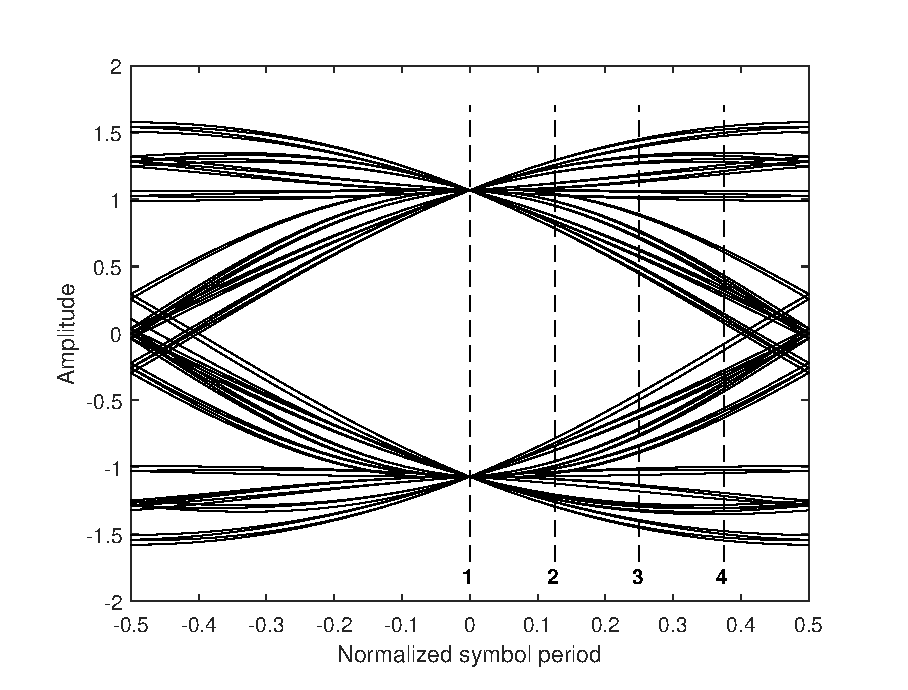
\includegraphics[width=3.1in]{pic/eye-ent-a-k.eps}}
% \hspace{0.2in} % 两图间距
\subfigure[Histograms of signal probability distribution]{
\label{fig:sig_prob}
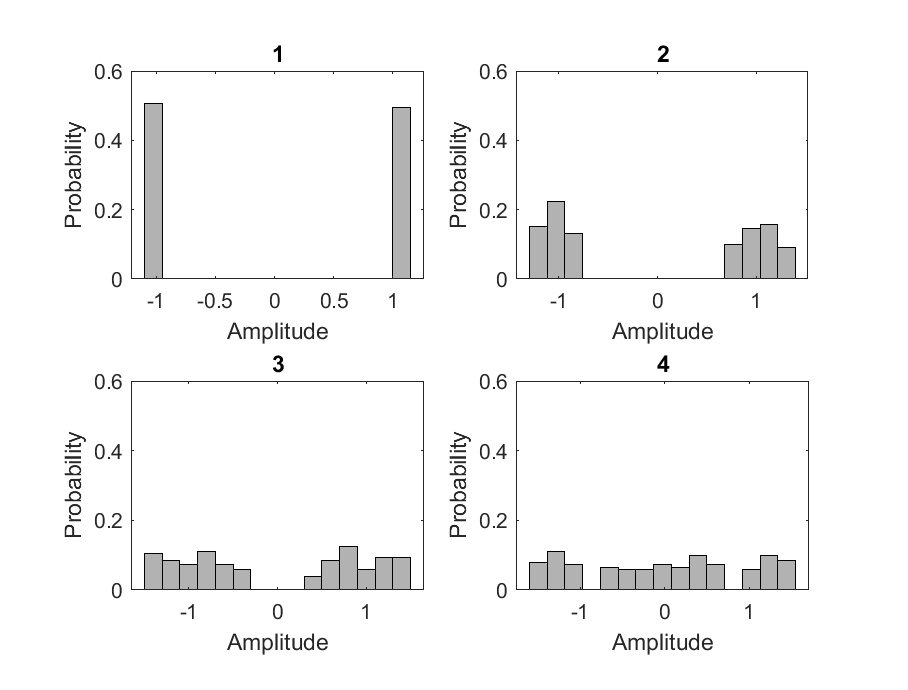
\includegraphics[width=3.1in]{pic/eye-ent-b-k.eps}}
\caption{Signal probability distribution on four timing instants on a typical eyediagram.}
\label{fig:eye_ent} %% 总 label
\end{figure}
% paper_plot.m

For example, a given modulation scheme with an alphabet size of \(M\) is implemented to transmit random data in an ideal channel. 
% An RC filter is applied for pulse shaping, and the channel is ideal.
% assuming no noise and perfect symbol timing (no ISI),
% The ISI can be eliminated if sampling in the middle of the eye diagram.
At the receiver, with perfect timing recovery, the signal samples can only be distributed equally within \(M\) possible symbols.
The probability that the samples belong to the $k$-th symbol is \(p_k=1/M\).
Substituting \(p_k\) into~(\ref{eq:entropy}), the minimum eye diagram entropy is defined as
\begin{equation}
\min{H_{eye}} =  - \sum\limits_{k = 1}^M {{\frac{1}{M}}\log_2 {\frac{1}{M}}}=\log_2 {M},
\label{eq:entropy_mid}
\end{equation}
which is exactly the same as the amount of information carried by each symbol.


The minimum eye diagram entropy only exists when the perfect symbol timing is achieved, because according to the Nyquist criterion, the ISI reaches zero at these timing instants.
If the sample distribution at a timing instant that deviates from the middle of the eye is examined, 
the Nyquist criterion is violated and the
interference from adjacent symbols increases the randomness.
% with different amplitudes will distort the .
% It is tedious to build an analytical relationship between the eye diagram entropy and the timing instant, but one intuitive explanation is given as follows.
A closed form of analytical relationship between the eye diagram entropy and the timing instant is difficult to demonstrate, however it can be observed that 
as the timing instant shifts away from the middle of the eye, the signal energy from current symbol decays, and the interference energy grows, leading to increased randomness.
% * <x.liu@dal.ca> 2018-02-02T03:12:10.862Z:
% 
% It is difficult to build an analytical relationship between the eye diagram entropy and the timing instant. Can we bypass it? same proof is needed in next section for frequency estimation
% 
% ^.
Therefore, the entropy being a measure of randomness will also increase accordingly.
Since each interference pulse from adjacent symbols carries the same amount of information, 
if the span of the pulse shaping filter is \(N_{span}\), 
the maximum eye diagram entropy will be \(N_{span}\) times the amount of information carried by each symbol, which can be presented as
% * <x.liu@dal.ca> 2018-02-06T17:35:48.137Z:
% 
% is this explanation clear enough?
% 
% ^.
\begin{equation}
\max{H_{eye}} =  N_{span}\log_2 {M}.
\label{eq:entropy_neb}
\end{equation}
% This maximum entropy is \(N_{span}\) times higher than the entropy measured in the middle of the eye diagram.
% There may be existence of local minima which will be addressed later in this paper,
% but one can conclude that the entropy of an eye diagram comes to a global minimum in the middle of the eye.

To summarize, the EM based symbol timing recovery seeks the timing instant with minimum eye diagram entropy. 
% The desired timing instant 
% The Nyquist criterion 
The eye diagram entropy can be seen as an indicator of the ISI that is introduced by the adjacent symbols.
Effectively, the  desired timing instant with zero ISI is the instant with minimum eye diagram entropy. 
% Therefore, the symbol timing recovery can be approached by searching the timing instant with the minimum eye diagram entropy.


\subsection{Constellation Diagram Entropy and Carrier Frequency Recovery}
\label{sec:const_entp}
The EM criterion can also be applied to recover the carrier frequency.
When the passband signal is down converted to baseband, the complex data can be visualized as a constellation diagram.
However, if the frequency of the local oscillator is  different (even by a very small margin) from the carrier of the signal, the resulting constellation diagram rotates and cannot be demodulated reliably.
The estimation of a CFO that is much smaller than the symbol rate is discussed in this section, since for a large CFO, a preceding coarse carrier recovery is usually required.


The randomness of the signal distribution on the constellation diagram can be quantitatively measured by the \textit{constellation diagram entropy}.
Similar to the eye diagram entropy, the histogram can be used for probability estimation.
However, a 2D histogram is needed to present both in-phase and quadrature components on the constellation diagram.
Examples of noise free QPSK constellation diagrams with zero, mild and strong CFO with their corresponding histograms are shown in Fig.~\ref{fig:const_hst}.
The constellation diagram entropy can be estimated with these 2D histograms.
According to~(\ref{eq:entropy}), the highest probability peaks in the histogram indicate the lowest entropy (as observed Fig.~\ref{fig:const_hst}(a)).
The probability that a sample occupies a given bin can be roughly considered to be equal in all bins. 
Therefore, it can be approximated by \(p_{const} \approx {1}/{n_{bin}}\), where \(n_{bin}\) is the number of histogram bins loaded with signal samples.
Thus, the constellation entropy is given by
\begin{equation}
H_{const} \approx - n_{bin} p_{const} \log_2 {p_{const}} \approx -\log_2 {\frac{1}{n_{bin}}}.
\label{eq:const_ent}
\end{equation}
For example, when the CFO is zero, \(\min{n_{bin}}=M\),  and the minimum constellation entropy is
\begin{equation}
\min{H_{const}=\log_2 {M}},
\end{equation}
which is the same as (\ref{eq:entropy_mid}).
There is also an upper limit on the constellation entropy 
when the rotation of the constellation results in samples that are uniformly distributed along a circle such that separate clusters can no longer be distinguished.  
% when the signal samples form a ``circle'' shape on the constellation diagram.
% * <x.liu@dal.ca> 2018-02-06T17:41:24.169Z:
% 
% I tried, but any reviewer can easily argue "no rigorous proof"
% 
% ^.
This phenomenon will be further discussed in Section~\ref{sec:carrier_recovery}.
Note that an analytical discussion is provided in \cite{Pedzisz2006} and demonstrates that, for PSK modulation,
the entropy has a global minimum and corresponds to a CFO equal to zero.
% , and its value is equal to the amount of the information carried by the symbol, which is the same as~(\ref{eq:entropy_neb}).
% The entropy maximum value is obtained when either the CFO or the number of samples are large enough,
% such that the accumulated signal phase error is greater than the minimum phase difference of the signal modulation scheme. 
% More discussion on entropy based carrier recovery can be found in \cite{Pedzisz2006}.

\begin{figure}[htbp]
\centering
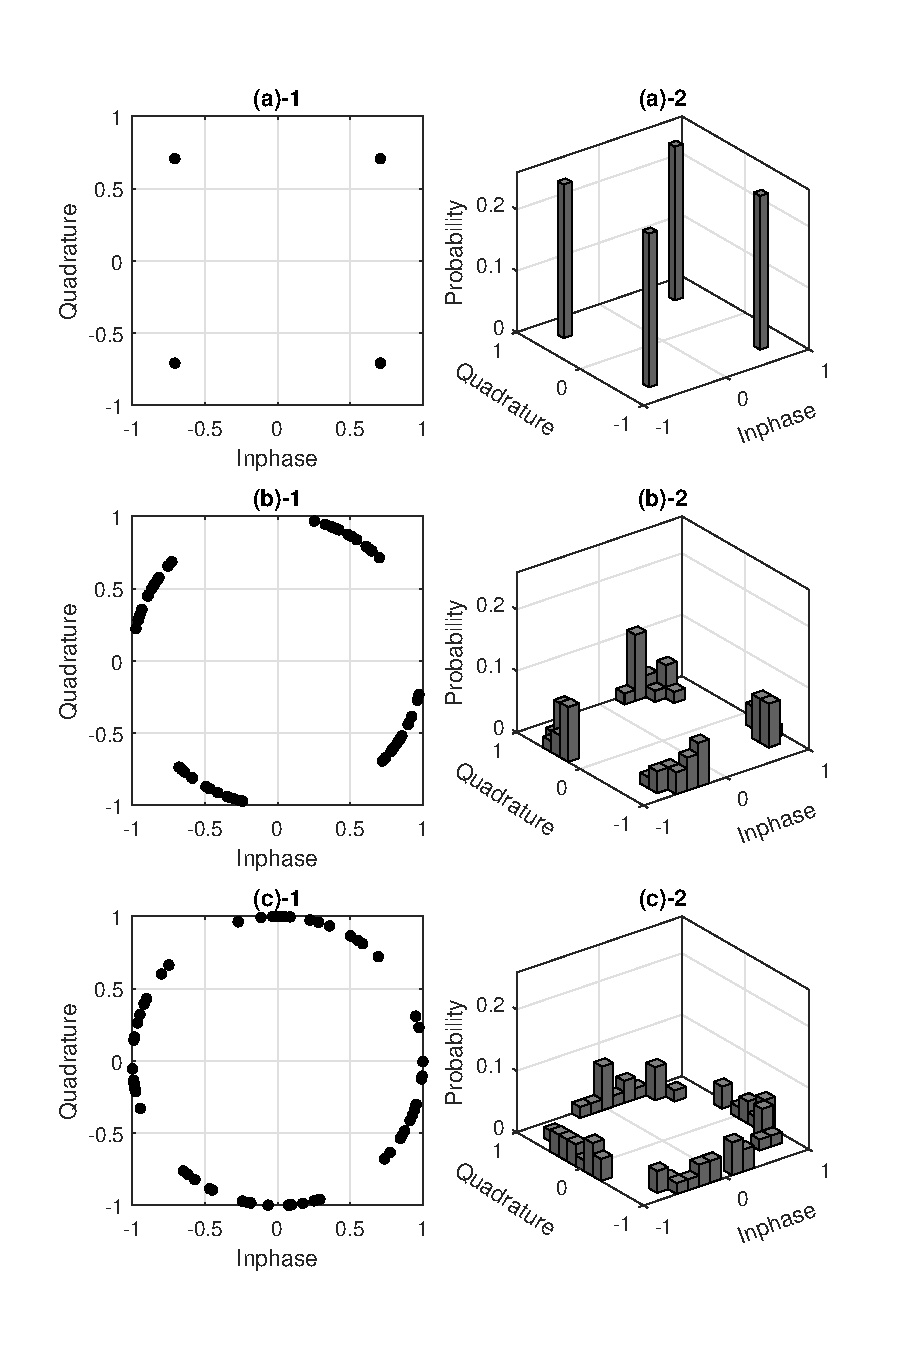
\includegraphics[width=3.5 in]{pic/const_hst-k.eps}
\caption{Constellation diagrams with different CFOs and the corresponding histograms of signal probability distribution.}
\label{fig:const_hst} 
\end{figure}
% paper_plot.m

% add content from my wuwnet paper
% The probability density function (PDF) of its instantaneous phase can be used to estimate the entropy, and with the help of
It is important to note that like the STO estimation, the CFO estimation can be achieved by searching the CFO with minimum constellation diagram entropy.
However, a global search for minimum entropy and the entropy estimation using a histogram are not efficient in practice.
In the next two sections, a methodology to implement this unified criterion is proposed.

\section{Customized Fast Entropy Estimation Algorithm}
\label{sec:cust_entp}
Entropy based algorithms are rarely used in signal processing because of their complexity~\cite{Bercher2000}.
% To develop practical entropy minimization based synchronization algorithms, a fast entropy estimation method is required.
% from the definition: histogram based estimation
According to the Shannon entropy defined by~(\ref{eq:entropy}), the entropy is a function of the probability of the samples.
A common technique is to use the histogram for probability estimation as shown in Fig.~\ref{fig:eye_ent} and Fig.~\ref{fig:const_hst}.
However, the estimation of the probability using a histogram and the summation of multiple logarithm operations  in~(\ref{eq:entropy}) have high computational complexity.
In this section, a fast customized entropy estimation algorithm that is suitable for EM based synchronization parameter estimation is propose. 

To reduce the entropy estimation complexity, alternative definitions of entropy have been proposed, such as the R\'enyi entropy.
The R\'enyi entropy  with an order \(\alpha\) is defined as \cite{renyi1961measures}
\begin{equation}
H_{R }={\frac {1}{1-\alpha }}\log {\Bigg (}\sum _{k=1}^{M}p_{k}^{\alpha }{\Bigg )}.
\label{eq:renyi}
\end{equation}
As explained in \cite{Bromiley2004}, when $\alpha~\to~1$, the R\'enyi entropy tends to be equal to the Shannon entropy.
Thus, the R\'enyi entropy is a generalization of the Shannon entropy.
The quadratic R\'enyi entropy ($\alpha=2$) is chosen in this work as suggested in~\cite{Santamaria2002}.
By replacing $\alpha$ in (\ref{eq:renyi}) with 2, the quadratic R\'enyi entropy is given as
\begin{equation}
H_{R2 }=-\log {\Bigg (}\sum _{i=1}^{M}p_{k}^{2 }{\Bigg )}.
\label{eq:renyi2}
\end{equation}
Note that in~(\ref{eq:renyi2}), the logarithm function is  external to the sum of the quadratic probabilities.
Because the logarithm function is monotonic, minimizing~(\ref{eq:renyi2}) is equivalent to maximizing its internal portion.
Since the search for a minimum entropy relies on a relative value of \(H_{R2 }\),
% only relative value is needed for searching a minimum entropy, 
the logarithm function can be dropped out without affecting the estimation result.
Recall Shannon entropy given in (\ref{eq:entropy}), the sum of \(p_k \log{p_k}\) is simplified to the sum of \(p_k^2\) here.
% * <x.liu@dal.ca> 2018-02-06T18:16:02.187Z:
% 
% do I clearly state why the logarithm can be dropped here?  
% 
% ^ <x.liu@dal.ca> 2018-02-21T20:33:37.631Z.

To obtain a relative \(H_{R2 }\), an inefficient histogram based probability estimation is still needed.
% To further investigate the argument of the logarithm function in~(\ref{eq:renyi2}), 
% a faster probability estimation method is required to replace the histogram based algorithm.
As suggested in~\cite{Principe2000a}, the \textit{kernel density estimation} (KDE) is a faster probability estimation method that can replace the histogram based algorithm.
It is also known as Parzen's window~\cite{Parzen1962} as one of the well-known non-parametric approaches to estimate the underlying probability of samples. 
% which is suggested in~\cite{Principe2000a}.
% is used to estimate the probabilities.
% * <x.liu@dal.ca> 2018-02-02T04:09:58.876Z:
% 
% OK I will talk about some background of the kernel method, why  and how to choose r 
% 
% ^ <x.liu@dal.ca> 2018-02-06T18:44:03.440Z.
Specifically, given a set of \(N\) samples, \(i=1, \dots, N\), the sample probability at an observation \(\xi\) can be estimated by
\begin{equation}
{ p(\xi)={\frac {1}{N}}\sum _{i=1}^{N}K_{r}\left(\xi-x_i\right)},
\label{eq:kde}
\end{equation}
where $K_r(\cdot)$ is a kernel function with a positive parameter $r$.
Then, by substituting (\ref{eq:kde}) into (\ref{eq:renyi2}) and after some simplification, we have
\begin{equation}
H_{R2 }=-\log {\Bigg (}\frac{1}{N^2}\sum _{i=1}^{N}\sum _{j=1}^{N}K_{r}\left(x_i-x_j\right){\Bigg )},
\label{eq:ker_ent_est}
\end{equation}
where \(p_k^2\) in (\ref{eq:renyi2}) is directly estimated by the kernel function.

Among various kernel functions, the Gaussian kernel is adopted in~\cite{Principe2000a}, but it can be further simplified to a top-hat kernel (at a cost of reasonable accuracy loss) to accelerate the computation. 
This kernel function is given by
\begin{equation}
{\displaystyle K_{r}(x)={\begin{cases}1,&|x|\leq r\\0,&{\mbox{otherwise.}}\end{cases}}}
\label{eq:tophat}
\end{equation}
where the threshold \(r\) is used to determine the quantization level in which samples are grouped for entropy estimation.
% if the two samples are closely located that can contribute to the entropy estimation.
The choice of \(r\) will be detailed later in this section.
% * <x.liu@dal.ca> 2018-02-06T19:19:10.431Z:
% 
% The choice of r is  explained here
% 
% ^ <x.liu@dal.ca> 2018-02-09T18:23:42.791Z.
Using~(\ref{eq:ker_ent_est}) and~(\ref{eq:tophat}), the entropy can be estimated by  measuring the distances between samples instead of using histograms.


With the discussion above, the proposed entropy estimation algorithm is summarized using the following steps:
\begin{enumerate}
\item For a given set of observations with $N$ samples, calculate all the distances \(d_{ij}\) between each sample pair \(x_i\) and \(x_j\), where \(1\le i<N\) and \( i<j \le N\). 
So \(d_{ij}\) is given by
 \begin{equation}
d_{ij}=\left\|x_i-x_j \right\|,
\label{eq:distance}
\end{equation}
where \(\left\| \cdot \right\|\) represents the Euclidean norm.
\item Define a threshold \(r\) and count the number of \(d_{ij}\) that satisfy $d_{ij}>r$, and denote the count as $H_{sp}$.
\item After normalization, express the modified R\'enyi entropy (MRE) as
\begin{equation}
H_{MRE}= \frac{ H_{sp}}{ N(N-1)/2}.
\label{eq:entorpy_ad}
\end{equation}
\end{enumerate}



% The last step normalizes $H_{sp}$, so that the modified R\'enyi entropy $H_{MR}$ does not depend on the number of samples.
The final result \(H_{MRE}\) is the modified version of the quadratic R\'enyi entropy in which the logarithm function is dropped.
% and in witch the kernel function is used for the probability estimation.
% We will call it the \textit{modified R\'enyi entropy} in the rest of the paper.
Because of the normalization, the value of $H_{MRE}$ is limited from 0 to 1 and is unitless.
This algorithm does not need to produce a histogram and does not need to compute the logarithm function, making it much faster than the histogram based conventional entropy estimation method.

% Another interpolation 
% In the study of physiological time series data, researchers use  approximate entropy (ApEn) \cite{Pincus1991}, or sample entropy (SampEn) \cite{Richman2000}. to estimate the complexity of the time series.
% Instead of estimating the probability of samples, theses algorithms are looking for the probability of new patterns.
% In practice, the entropy increases for newer patterns. 

An example of the MRE estimation of a constellation diagram as a function of SNR is shown in Fig.~\ref{fig:MRE}, where the 2D histogram based Shannon entropy results are also plotted as a reference.
The samples are QPSK modulated with unit amplitude and perfect synchronization.

\begin{figure}[ht]
\centering
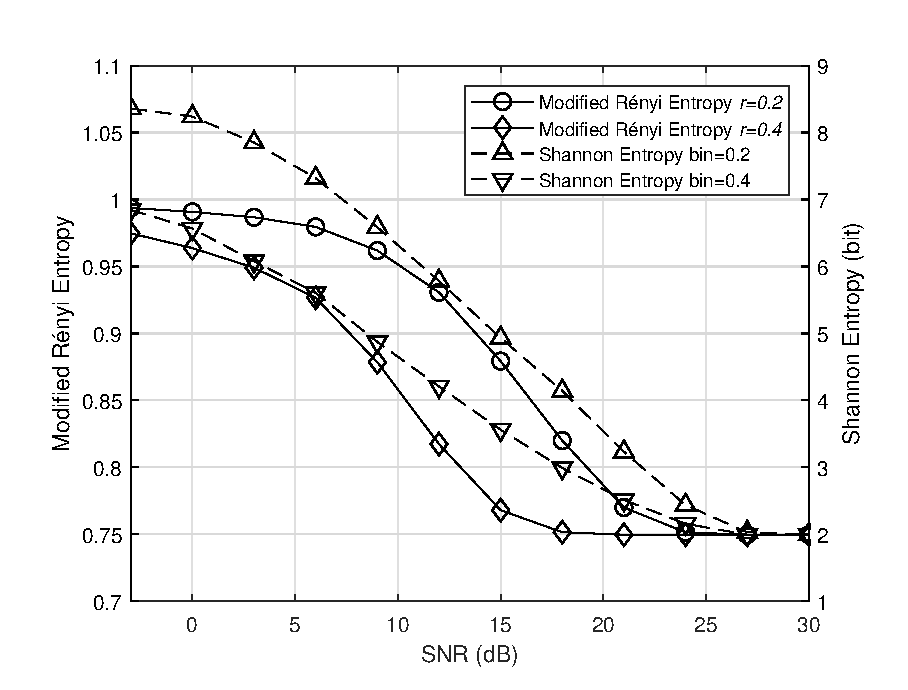
\includegraphics[width=3.1 in]{pic/MRE-k.eps}
\caption{Entropy estimation using two algorithms.}
\label{fig:MRE} 
\end{figure}
% The additive white Gaussian noise (AWGN) is introduced, where the SNR sweeps from -3 dB to 30 dB.

In Fig.~\ref{fig:MRE}, the thresholds \(r\) used in the MRE estimation are equal to 0.2 and 0.4, which are 20\% and 40\% of the symbol amplitude. 
% Its entropy estimate results are normalized and scaled such that it can share the same y-axis with MRE.
The histogram based estimation is evaluated with a bin width that is equal to the threshold \(r\).
% The threshold values \(r\) used in the MRE estimation are equal to the bin widths.
Both entropy estimation results can be found to be monotonic functions of SNR.
% It can be seen that both algorithms decrease monotonically with SNR.
The decreasing entropy reflects the fact that the uncertainty of the system is reduced with the increasing SNR.
This property shows that the proposed algorithm can be used to measure the data randomness.
When the SNR is sufficiently high, the Shannon entropy reaches the minimum. 
Its value is 2 bits, as predicted by~(\ref{eq:entropy_mid}).

The minimum value of the MRE can be derived and compared with the numerical results shown in Fig.~\ref{fig:MRE}.
Since the symbols are random, there are four groups of symbols distributed in the constellation diagram, such that each group has \(N/4\) samples.
The condition of $d_{ij}>r$ can only be satisfied between samples with different constellation positions.
If two of these constellation positions are considered, we have $H_{sp} = (N/4)^2$, so the total $H_{sp}$ will be $6 (N/4)^2$ if all four constellation positions are considered.
Thus, the minimum value of the MRE is approximated by
\begin{equation}
\min{H_{MRE}} \approx \frac{ 6 \left(N/4\right)^2}{N^2/2}=0.75,
\label{eq:adEntQPSK}
\end{equation}
which agrees with the results shown in Fig.~\ref{fig:MRE}.




The choice of the threshold \(r\) (sometimes referred as bandwidth~\cite{Botev2010}) exhibits a strong influence on the results.
It can be derived arithmetically from sophisticated algorithms to achieve an optimal probability estimate~\cite{Botev2010}.
% The rule of thumb for the choosing of threshold \(r\) depends mainly on the noise level.
In Fig.~\ref{fig:MRE}, the curve with \(r=0.2\) reflects randomness at high SNR, but saturates in the low SNR region, in which case \(r=0.4\) is preferred.
This behaviour is observed because when the \(r\) is small, the algorithm cannot accurately quantify the degree of aggregation of large scale distributed data samples.
In our application, the accurate absolute entropy value is not important, and the threshold $r$ is set equal to the root-mean-square value of the noise.
% inaccurate probability value is not a issue, since a STO or CFO with minimum entropy is what we actually need to search for.
% Empirical, $r$ is set equal to the root-mean-square value of the noise.

Another design parameter for MRE estimation is the number of samples, which is set equal to a few hundred in our application.
Entropy estimation is more accurate with a growing number of samples, but the number of distance calculation grows quadratically.
% growth with number of data samples. 
The computational complexity can be relieved by 
% either skipping the distance calculation of aggregated samples or 
using other distance metrics (Chebychev et al. \cite{Cha2007}).
However, it will cause a reduced tracking ability, which means that the algorithm cannot adapt to the time varying channel effectively.
As such, the choice for the number of samples depends both on the dynamic channel conditions and the hardware capabilities.
% this is not an issue in our application since a reliable synchronization  recovery with less data samples is always preferred, and it is an advantage in tracking the dynamic channel conditions. 
% * <x.liu@dal.ca> 2018-02-06T19:39:23.158Z:
% 
% I don't know how to make rigorous treatment for r and number of samples in these two paragraphs. they are more empirical parameters to me, sadly 
% 
% ^.

%%%%%%%%%%%%%%%%%%%%%%%%%%%%%%%%%%%%%%%%%%%%%%%%%%
\section{Implementation of Symbol Timing and Carrier Frequency Estimation}
\label{sec:imple}
In this section, the EM criterion will be implemented for symbol timing and carrier frequency estimation.
Practical issues are addressed and the estimation algorithms are discussed in detail. 
% The algorithms discussed here work in batch mode, which means the samples are processed block by block. 
% It is a direct result of the way entropy is estimated, however, after the initial acquisition, it is not difficult to adapt the algorithms to online mode with a sliding window.
% EM based symbol timing and carrier frequency recovery algorithms
% - configuration: batch search algorithms, timing first and then carrier recovery

\subsection{Symbol Timing Estimation} 
\label{sec:timing}
Symbol timing estimation can be implemented by searching for the instant with minimum entropy in the eye diagram.
% However, there are several practical issues that need to be addressed.
% In the following discussion, we will focus on:
In this section, the following practical issues are addressed:
1)~resolving local minima in the entropy curve,  
2)~examining the timing recovery in presence of CFO, and 
3)~providing accurate STO estimation at low oversampling rate.

The entropy reaches a global minimum in the centre of the eye diagram, but in practice, when the timing instant is close to the symbol transition area, the entropy may decrease and create local minima. 
Local minima deteriorate the performance at low SNR conditions, and particularly if gradient based search algorithms are used.
Since the entropy local minima occur when the sample magnitude is small, 
an additional threshold can be introduced to eliminate these data samples in the entropy estimation.
The following steps summarize an improved algorithm compared to that described in Section~\ref{sec:cust_entp}.
% The procedure is summarized using the following steps.
% With this idea, the algorithm in Section~\ref{sec:cust_entp} is amended:

\begin{enumerate}
\item Define a threshold \(r_{mg}\) and build a new sample set where all samples with a magnitude greater than \(r_{mg}\) are included.
The number of samples in the new set is denoted as \(N_{mg}\).
\item Find all the Euclidean distances \(d_{ij}\) between each sample pair \(x_i\) and \(x_j\) in the new sample set, where \(1\le i<N_{mg}\) and \( i<j \le N_{mg}\). 
\item Define a threshold \(r\). Count the number of \(d_{ij}\) such that $d_{ij}<r$, and denote it as $H_{ag}$.
\item Express the bounded modified R\'enyi entropy (BMRE) as
\begin{equation}
H_{BMRE}= 1- \frac{ H_{ag}}{ N(N-1)/2}.
\label{eq:entorpy_ad2}
\end{equation}
\end{enumerate}



A typical case is given here to show how the EM based STO estimation works.
The received signal consists of a frame of QPSK modulated random symbols, 
which are pulse shaped to generate a baseband complex envelop.
The oversampling rate is 40 to provide a better eye diagram resolution.
An AWGN channel is assumed with $E_s/N_0 = 18~\text{dB}$. 
After the matched filter, the eye diagram of the real component of the signal is shown in the upper part of Fig.~\ref{fig:timing}, and both the BMRE and MRE estimation results are shown in the lower part,
% the entropy results estimated by both original and modified algorithms are shown in the lower part,
% as well as its entropy are plotted in , where
where the thresholds are fixed to $r=0.25$ and \(r_{mg}=0.3\).


\begin{figure}[htbp]
\centering
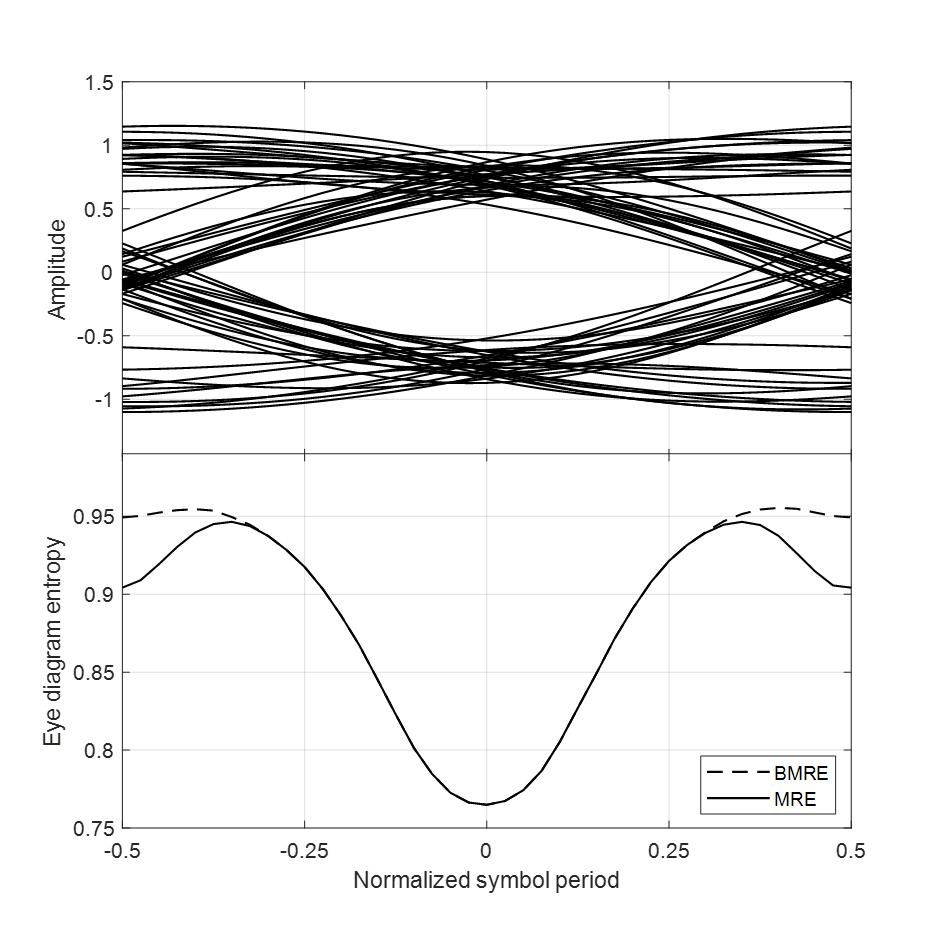
\includegraphics[width=3.1 in]{pic/timing.png}
\caption{An typical eye diagram (upper) and the corresponding eye diagram entropy (lower).}
\label{fig:timing} 
\end{figure}

% \subsection{Entropy Local Minimum Removal}
In Fig.~\ref{fig:timing}, the entropy reaches a global minimum in the centre of the eye diagram, and its value is close to 0.75 as predicted by~(\ref{eq:adEntQPSK}).
% With an increase of timing offset, 
The entropy increases with the absolute value of STO, indicating  more randomness introduced by ISI.
When the timing offset is beyond $\pm 0.35$, the  entropy from the MRE estimation decreases and creates a local minimum in the symbol transition area. 
This phenomenon is also illustrated in the eye diagram, where the samples aggregate into three visible groups (with amplitudes of \(\pm 1\) and 0).
% The local minimum is not a big issue if the SNR is high and a global search is applied, but it will deteriorate the performance in low SNR cases or when using gradient based search algorithms.

% The ad-hoc entropy estimated by the modified algorithm is also plotted in the lower part of Fig.~\ref{fig:timing} where the \(r=0.25\).
The result of the BMRE algorithm coincides with that of the original MRE algorithm in most of the timing instants, but the local minima near $\pm0.5$ become flat.
As such, with the BMRE estimation algorithm, the local entropy minima due to the symbol transitions are removed, and the STO can be estimated with higher accuracy.

% \subsection{Timing Recovery with Carrier Frequency Offset}
% In Fig.~\ref{fig:sysconf}, the timing recovery block is placed before carrier recovery, so the input signal of timing recovery may contain uncompensated CFO.
% We shall evaluate the viability of the proposed algorithm in such conditions. 
Next, the impact of timing recovery in presence of uncompensated CFO will be evaluated.  
Theoretically, the previous analysis of eye diagram entropy still holds, but the CFO does introduce extra entropy in the estimation.
To understand how the CFO affects the eye diagram entropy, another simulation is conducted with the parameters similarly to what was demonstrated in the early part of this section,
and the only difference is that a CFO at 1\% of symbol rate is introduced.
The eye diagram and the corresponding entropy are depicted in Fig.~\ref{fig:timing_freq}.
      
\begin{figure}[ht]
\centering
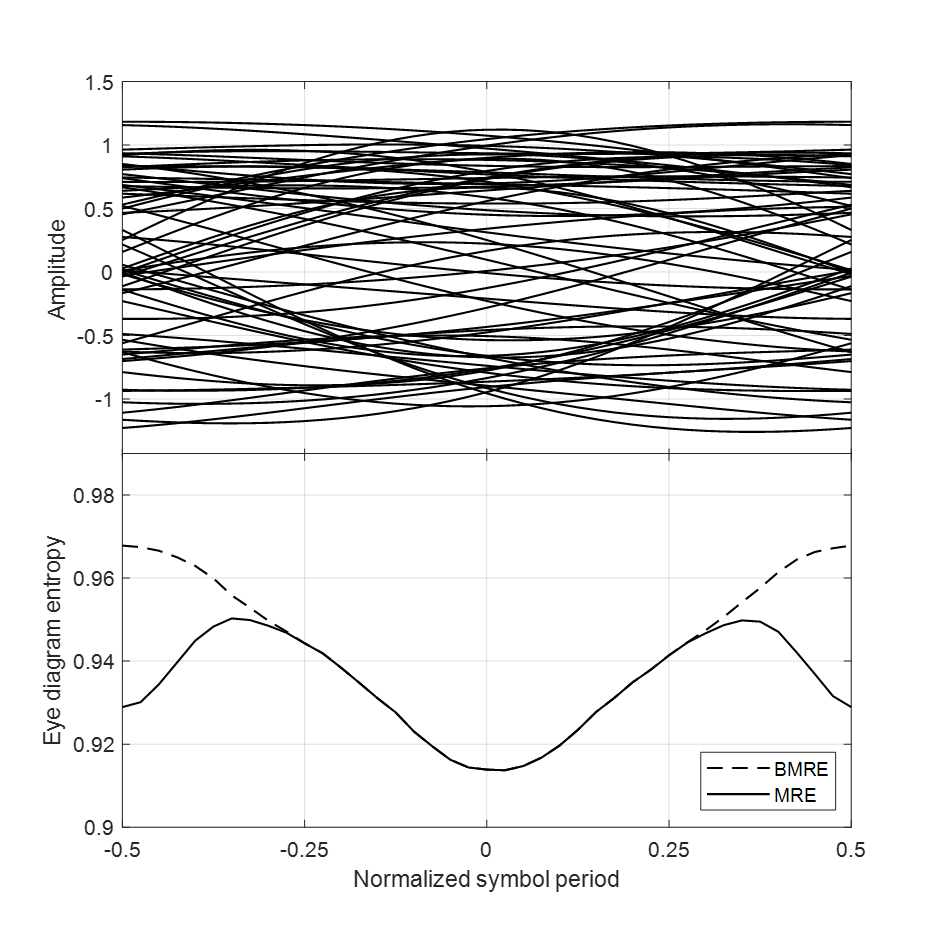
\includegraphics[width=3.1 in]{pic/timing_freq.png}
\caption{An eye diagram with carrier frequency offset (upper) and the corresponding eye diagram entropy (lower).}
\label{fig:timing_freq} 
\end{figure}

The eye diagram shows an eye that is completely closed: the centre of the eye or optimum timing instant cannot be identified by only looking at the eye diagram.
However, the optimum timing instant can be clearly identified with the entropy curve.
Both the MRE and the BMRE algorithms have the same global minimum at zero STO. 
Effectively, the eye diagram entropy based algorithm can detect the STO accurately,
but with a smaller entropy range than that without CFO.

It is also interesting to observe the entropy plot at a symbol transition in Fig.~\ref{fig:timing_freq}.
With the MRE algorithm, the local minima are more noticeable and may lead to a false STO estimate.
However, the BMRE algorithm shows superior performance:
the curve is not flat anymore but continues growing with the same gradient as a function of timing offset.
This feature shows a good adaptation of the BMRE algorithm, and proves that the ``symbol timing before carrier recovery'' configuration is feasible.


The last issue that will be addressed in the symbol timing recovery is the STO estimation for signals with low oversampling rate.
In the previous discussion, a global search for STO with minimum eye diagram entropy requires a high oversampling rate (normally more than 10 samples per symbol).
However, this is not always available in practice, especially for high speed communication.
% is not an elegant solution, especially when a high oversampling rate is not available.
Recall that 
% the widely used feedforward symbol timing method,
the O\&M algorithm uses as low as 4 samples per symbol, and its STO is given by
\begin{equation}
\tau=\frac{T}{2\pi}\arg \left\{ {\sum\limits_{i = 1}^{N} {x_i^2{e^{ - j2\pi (i-1)/N_{sps}}}} } \right\},
\label{eq:om}
\end{equation}
where \(T\) is the symbol period and \(N_{sps}\) is the oversampling rate.
The operation \(\arg( \cdot )\) returns the phase angles in radians.
The guiding principle of the O\&M algorithm is to apply a discrete Fourier transform (DFT) to the squared signal \(x_i^2\),
and the STO is extracted from the angle of the resulting spectrum line at the symbol rate.

The theory behind (\ref{eq:om}) is that the squared signal \(x_i^2\) is a periodic signal with the same frequency and phase as the pulse shaped symbols due to the cyclostationary property of \(x_i\).
Thus, even with a low oversampling rate, the STO can still be estimated by DFT.
The eye diagram entropy curve exhibits a similar property as \(x_i^2\) within one period,
therefore, the same approach can be applied to the EM based symbol timing algorithm.
% * <x.liu@dal.ca> 2018-02-10T17:50:22.606Z:
% 
% did I explain it clearly?
% 
% ^ <x.liu@dal.ca> 2018-02-27T14:07:49.760Z.
To be specific, \(x_i^2\) in~(\ref{eq:om}) can be replaced  with the eye diagram entropy \(H_i\), 
such that the STO can be found with
\begin{equation}
\tau  = \frac{T}{{2\pi }}\arg \left\{ {\sum\limits_{i = 1}^{N_{sps}} {H_i{e^{ - j2\pi (i-1)/N_{sps}}}} } \right\}.
\label{eq:ff_alg}
\end{equation}
% where \(H(k)\) is the eye diagram entropy at timing instant \(k\).
Note that (\ref{eq:ff_alg}) assumes that the entropy curve is symmetric to the centre of the eyediagram,
but the symmetry may not be maintained at low SNR or in a multipath channel.
% Application of this algorithm in such conditions may result in large estimation variance.
In these conditions, the algorithm may result in large estimation variance.
% Therefore, a global search is still preferred in these conditions.
% Its performance will be further discussed in Section \ref{sec:perfo}.

\subsection{Carrier Frequency Estimation}
\label{sec:carrier_recovery}
In this section, the implementation of the EM based CFO estimation algorithm is detailed.
Similarly to the STO estimation discussed above, the proposed algorithm is also NDA.
The constellation diagram entropy is measured by defining an adequate range for the trial CFO, and a global search is applied to find the minimum entropy. 
% The general idea is to multiply the signal by a local carrier with a trial CFO and calculate the corresponding constellation entropy.
% Then, sweep the trial CFO in a certain range and find the frequency with the minimum entropy value.
The characteristics of the entropy curve are shown first and then a method that can increase the global search efficiency is proposed. 
% reduce that number of trials required to obtain a global minimum.

In Section \ref{sec:const_entp}, it is observed that the constellation entropy is almost flat when the CFO is greater than a frequency limit.
Within this frequency limit, the curve has a V-shape ``trough'' (negative peak) and the entropy global minimum is located in the middle of the trough.
For a given modulation scheme, the range of the trough is affected by the CFO ($f_\Delta$), the symbol rate $1/T$, and the number of data samples $N$ in the window.
For example, the \(M\)-PSK modulated signal has a minimum constellation phase difference \(2\pi/M\).
The accumulated phase shift due to CFO is given by \(2\pi f_\Delta N T\).
The constellation entropy increases with the CFO until the accumulated phase shift is greater than the minimum constellation phase difference. 
Therefore, the trough range is given by
\begin{equation}
\left| {f_\Delta } \right| < \frac{1}{{MNT}},
\label{eq:freq_limit}
\end{equation}
\noindent and when the CFO is larger than $1/MNT$, the entropy curve becomes flat.


In (\ref{eq:freq_limit}), if \(N\) is equal to a few hundred samples, a given CFO that can fall into the entropy trough has to be on the order of 0.1\% of the symbol rate, which is relatively small compared to the CFO range that needs to be covered.
The resulting entropy curve as a function of trial CFO is generally flat with the exception of a sharp trough.
A similar result has also been reported in~\cite{Pedzisz2006}. 
Consequently, the linear search requires very fine steps to achieve high frequency resolution, and the potential gradient descent algorithm may not converge due to lack of gradient.
In other words, an efficient search algorithm cannot be applied. 

In order to cover a large estimation range without intensive computation, an algorithm that can expand the width of the trough is required.
% One possible way that can obtain a wide entropy trough
To increase the trough width, a possible solution is to reduce \(N\).
However, this will lead to an inaccurate PDF and entropy estimation.
Instead, a block average algorithm inspired by~\cite{YuanlingHuang2007} is adopted to smooth the entropy curve. The algorithm is realized using the following steps:

\begin{enumerate}
\item Segment the \(N\) data samples into small blocks equally, where each of these block consists of \(L\) samples. 
% There can be overlaps for the blocks to improve the accuracy.
\item Estimate the entropy curve for each block.
\item Average the entropy results from all the blocks.
\end{enumerate}
If the CFO is constant through all the data samples, each block should possess the same entropy curve but with random fluctuation since only a small number of samples are available for probability estimation.
% due to PDF estimation with insufficient samples.
By averaging the entropy curve using small blocks, a wide and smooth entropy trough is achieved.
The new trough is $N/L$ times wider than the original one.

With the same settings as in Section \ref{sec:timing}, the numerical simulation of the constellation entropy is compared using 400 samples, 50 samples and block averaging 400 samples with a block size of 50 samples.
% as well as for the entropy with block averaging. 
The results are plotted as a function of the CFO in Fig.~\ref{fig:freq_entp}.
Perfect symbol timing is assumed, and the CFO is swept within 1\% of the symbol rate.

% The frequency offset under recovery should be smaller than the symbol rate \cite{mengali1997synchronization}.
% To be specific, for \(M\)-PSK modulation schemes, if there are \(N\) samples with sampling interval of \(T_s\), the upper boundary of the frequency offset \(\Delta \omega_c\) is given by
% \begin{equation}
% \Delta \omega_c <\frac{2 \pi}{M N T_s}  
% \label{eq:f_lim}
% \end{equation}
% Regarding the case of QAM signals, the \(2 \pi/M\) in (\ref{eq:f_lim}) should be replaced by the minimum phase difference between their constellation points.

% \subsection{}

\begin{figure}[ht]
\centering
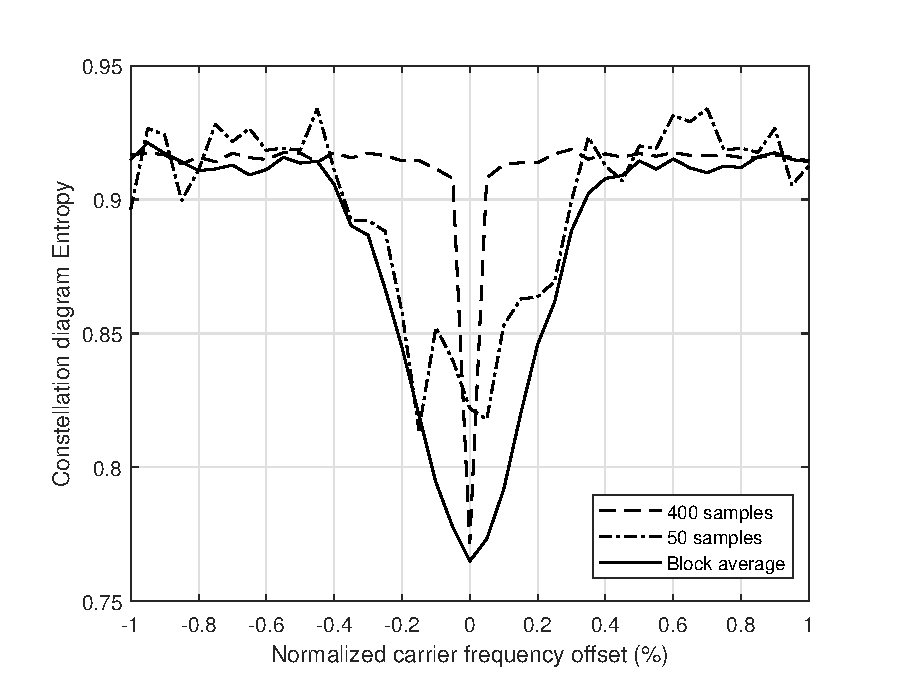
\includegraphics[width=3.1 in]{pic/freq-k.eps}
\caption{Constellation diagram entropy for carrier frequency recovery.}
\label{fig:freq_entp} 
\end{figure}   
% carrier_entropy.m

% \subsection{Entropy Curve Expansion}
As can be observed in Fig.~\ref{fig:freq_entp}, the entropy curve using 400 samples has only one global minimum when the CFO is equal to zero and no other local minimum.
But its curve has a very narrow trough as predicted.
In comparison, the entropy estimated using 50 samples has a trough boundary at \(\pm 0.5\%\) of the symbol rate, which agrees with (\ref{eq:freq_limit}).
In fact, the trough range is expanded 8 times, but many fluctuations and local minima appear.
The entropy curve using the block averaging has the same expanded trough as the entropy estimated using 50 samples, but with a smooth gradient and without any local minimum.

Given the expanded entropy trough, a more efficient two-step linear search can be readily applied.
First, a coarse search through the frequency range of interest with step size equal to the half trough width can provide an approximate CFO estimate.
A second search with a fine frequency step near the coarse estimation result can improve the accuracy of the CFO estimate.

Recall that the computation complexity grows quadratically with the number of samples, so breaking down the sample set into small blocks can significantly reduce the required computation.
For example, if the 400 samples are equally divided into 8 blocks, it is easy to find that compared to the algorithm without block averaging, 
this algorithm requires eight times less number of Euclidean distance calculations (defined by~(\ref{eq:distance})). 
This is a significant reduction in computational complexity. 

% These EM based synchronization algorithms will be tested in controlled and realistic conditions in the nest section.

% In the above discussion, the CFO in each data batch is estimated and compensated,
% but the phase is not considered and there is phase discontinuity between batches.
% The initial phase of the data batch should be aligned with the last batch to ensure the phase continuity before the following carrier recovery.

% \subsection{Carrier Phase Continuity}
%     - only carrier frequency is recovered, phase different between blocks
%       - keep phase continuity between blocks

% \textbf{to be continued...}
% In high data-rate cases, the synchronization parameters
% (ε, θ, ω) vary slowly in comparison with the symbol interval.
% They can be assumed piecewise constant over a number of
% symbol periods. Synchronization of these quasi-constant parameters
% will be considered here, while tracking of the slowly
% varying parameters can be done in a post-processing unit [3].
%%%%%%%%%%%%%%%%%%%%%%%%%%%%%%%%%%%%%%%% The effect of various channel impairments will be analyzed on the system performance.  
%%%%%%%%%%
\section{Performance Evaluation}
\label{sec:perfo}
In this section, the performance of the symbol timing and carrier frequency estimation algorithms presented in the previous section are assessed in controlled conditions.
% In Section~\ref{sec:per_sim},  
The estimation variances using EM and ML algorithms in AWGN channel are compared.
Also, the effect of multipath impairment is analyzed on the system performance.
% , including noise, timing with CFO as well as multipath 

% Finally, to examine the EM algorithm in realistic time varying channels, in Section~\ref{sec:per_sea}, it is applied to a set of underwater acoustic communication data taken during a sea trial.

% \section{Timing Recovery Performance}
% \section{Numerical Simulation}
% \label{sec:per_sim}
% \section{Symbol Timing Performance}
First, the performance of the symbol timing estimation algorithm (\ref{eq:ff_alg}) is examined in presence of AWGN.
The O\&M algorithm
% is a batch mode, feedforward symbol timing estimator as 
described by (\ref{eq:om})
% with the same structure as the proposed timing recovery algorithm~(\ref{eq:ff_alg}), 
% Therefore, it 
is used here to represent the ML estimator for comparison.

The performance comparison in presence of AWGN is shown in Fig.~\ref{fig:timing_per}.
In this figure, both QPSK and 16-QAM modulation are evaluated.
A pulse shaping filter is used to limit the bandwidth.
% The RRC filter has a rolloff factor of 0.25. 
AWGN is added to the received signal, such that the symbol energy to noise spectral density ratio (\(E_s/N_0\)) ranges from 5 to 40~dB. 
% with a step of 5~dB.
For each \(E_s/N_0\) setting, 500 Monte Carlo trials are conducted.
In each trial, a block size of 100 samples are used to estimate the STO.
After normalization by the symbol period, the timing error variances are represented in the figure.
% It is necessary to compare the results with the theoretical limit.
Following \cite{mengali1997synchronization}, the modified Cram\'er-Rao bound (MCRB) is also shown as the theoretical limit.

\begin{figure}[ht]
\centering
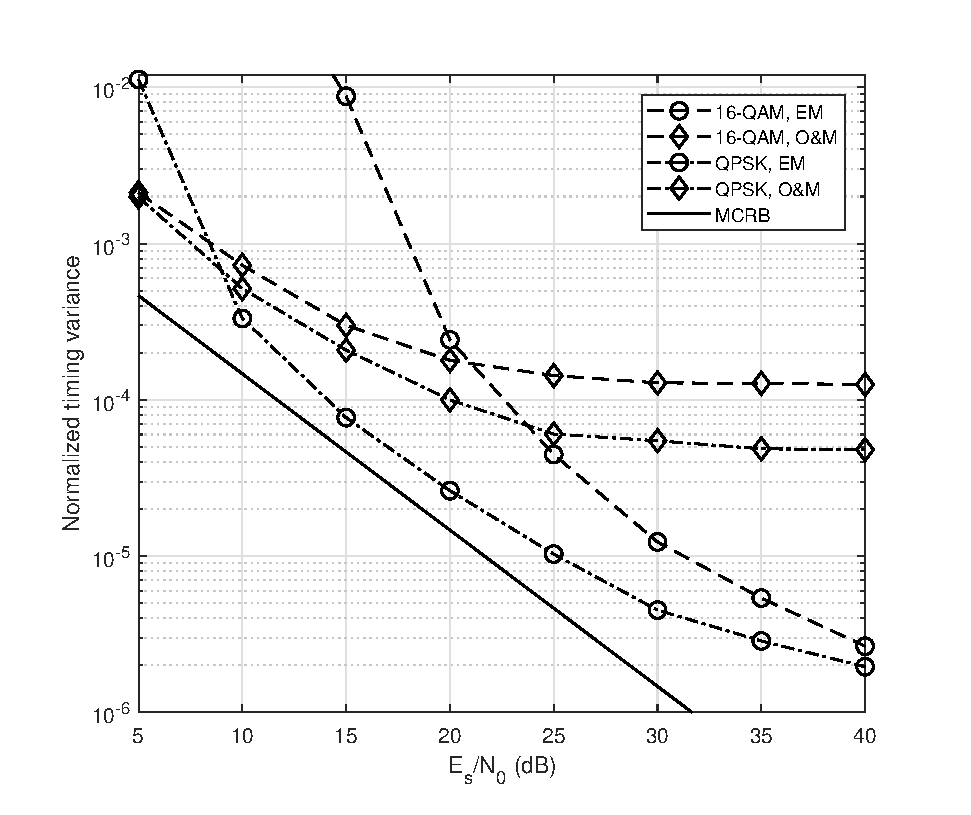
\includegraphics[width=3.1 in]{pic/per_timing-k.eps}
\caption{Performance of two symbol timing algorithms with 16-QAM and QPSK modulation schemes.}
\label{fig:timing_per} 
\end{figure}   
% MCRB_timing_nda3.m

Several conclusions can be draw from this figure.
Generally speaking, when the  \(E_s/N_0\) is sufficiently high, the EM based symbol timing algorithm has lower variance than the O\&M algorithm for both QPSK and 16-QAM modulation schemes.
% This transition \(E_s/N_0\) is 8~dB for QPSK and 27~dB for 16-QAM
For both algorithms, the low modulation order tends to yield smaller timing variance.
% In the high \(E_s/N_0\) region, the performance of O\&M algorithm is limited by the self noise. 
When the \(E_s/N_0\) is greater than 25~dB, the O\&M reaches a lower boundary because of its strong self noise~\cite{mengali1997synchronization}. 
% * <x.liu@dal.ca> 2017-10-27T13:27:20.450Z:
% 
% the self noise is actually ISI, but they used this term in the citation to differentiate thermal noise
% 
% ^.
% When the \(E_s/N_0\) is greater than 25~dB, the strong self noise due to the small rolloff factor makes O\&M algorithm reaches its lower boundary, while 
In contrast, the performance of the EM algorithm keeps on improving with \(E_s/N_0\), since its timing variance keeps getting smaller with the increased \(E_s/N_0\).
However, in the low \(E_s/N_0\) region (lower than 21~dB for 16-QAM and 9~dB for QPSK), the EM algorithm has inferior performance compared with the O\&M algorithm.
This is because the O\&M algorithm, as an example of ML algorithms, is designed under AWGN assumption, while the EM algorithm is more suitable when the ISI dominates.


Note that in the simulation, a pulse shaping filter with a small excess bandwidth of 25\% is used at the expense of excessive ISI.
% the rolloff factor is 0.25, which means the signal occupies relative small bandwidth but with significant ISI.
In this situation the EM based algorithm is favoured, because the eye diagram entropy estimation can effectively measures the ISI.
However, if a pulse shaping filter with larger excess bandwidth is used, the O\&M algorithm will have a performance very close to the MCRB~\cite{mengali1997synchronization}.
% * <x.liu@dal.ca> 2017-10-27T14:11:51.042Z:
% 
% at of the?
% 
% ^.
% On the other hand, the enlarged signal bandwidth and reduced ISI make the EM based algorithm have inferior performance than the O\&M algorithm.

% \textit{Experiment 2: Performance of the symbol timing recovery in the presence of CFO.}
As explained in Section \ref{sec:timing}, the EM based symbol timing estimation is insensitive to the CFO, but it is interesting to understand how the performance changes in the presence of CFO. 
The simulation settings are generally the same as for the last one, except that different modulation schemes, BPSK and QPSK,  are evaluated here.
The introduced CFO is 1\% of the symbol rate, and the timing variances are plotted in Fig.~\ref{fig:timing_frq_per}.

\begin{figure}[ht]
\centering
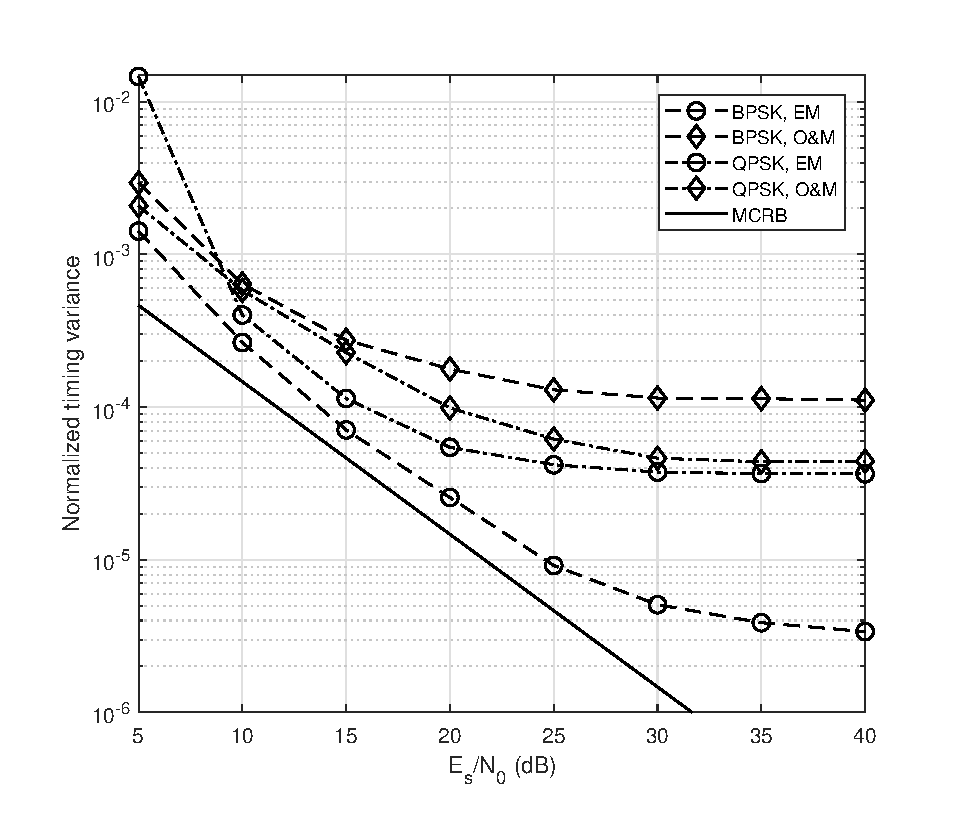
\includegraphics[width=3.1 in]{pic/per_timing_frq-k.eps}
\caption{Performance of two symbol timing algorithms in the presence of CFO.}
\label{fig:timing_frq_per} 
\end{figure}  
% MCRB_timing_nda4.m

For BPSK modulation, the EM based algorithm shows good performance that is close to the MCRB when the \(E_s/N_0\) is below 30 dB.
It has the highest performance improvement compared to the O\&M algorithm.
However, for QPSK modulation, the performance improvement is marginal.
This is because, for the EM based algorithm in (\ref{eq:ff_alg}), it is assumed that the eye diagram entropy curve is symmetrical to the centre of the eye diagram, and this only stands with low modulation order and low noise level.
Another example of an asymmetrical eye diagram entropy condition will be analyzed in the following simulation. 

% \textit{Experiment 3:EM based symbol timing recovery in multipath channel.}
A key issue that coherent communication systems are facing is the multipath channel impairment.
Unpredictable channel impulse responses violate the Nyquist ISI criterion, and the communication performance is compromised.
The nature of EM based symbol timing estimation is to search for timing instant with minimum ISI, which makes it more suitable for these conditions than ML based algorithms.
To demonstrate this, a set of BPSK modulated signal with 50\% excess bandwidth is used as the transmit data.
For simplicity reason, a multipath channel considered here has one direct path (with an amplitude normalized to 1 and arrival time at 0) and two indirect paths.
Its impulse response $h(t)$ is given by
% \begin{equation}
% h(t)=\delta(t)+0.6\delta(t-1.6T)-0.3\delta(t-2.1T).
% \label{eq:multi_path}
% \end{equation}
\begin{equation}
h(t)=\delta(t)+0.5\delta(t-1.4T)+0.2\delta(t-3.5T).
\label{eq:multi_path}
\end{equation}
% \noindent where the second tap is a fraction of the symbol period.  
At the receiver, the eye diagram and the timing instants estimated by both O\&M and EM algorithms are plotted in Fig.~\ref{fig:per_timing_isi} for \(E_s/N_0\) equal to 15 dB. 
% code: multi_path_new.m
\begin{figure}[ht]
\centering
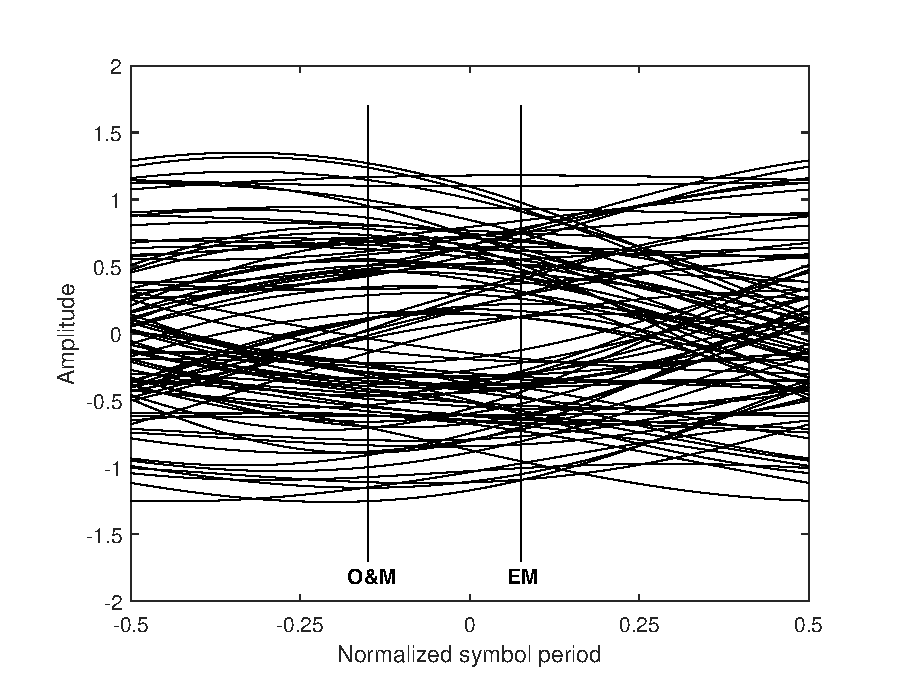
\includegraphics[width=3.1 in]{pic/per_timing_multi-k.eps}
\caption{An eye diagram after a multipath channel and the corresponding timing estimation results.}
\label{fig:per_timing_isi} 
\end{figure} 
% multi_path_new.m

The eye diagram in Fig.~\ref{fig:per_timing_isi} is almost closed and shifted from the centre due to ISI.
The bit error rates (BER) of demodulated samples recovered by the two algorithms are compared without equalization.
The EM algorithm can find the maximum eye opening and achieve a BER of 1.2\%.
In contrast, the BER is 5.9\% if STO estimation using the O\&M algorithm and 1.4\% when sampling in the middle of the direct arrival.
As one can observe in Fig.~\ref{fig:per_timing_isi}, the samples recovered by the O\&M algorithm have the highest energy output, but with strong ISI.

The results from channel given by (\ref{eq:multi_path}) is not a special case.
Consider a general form for a three-path channel
\begin{equation}
h(t)=\sum\limits_{n = 1}^{3}{a_n\delta(t - b_n T)},
\label{eq:multi_path_2}
\end{equation}
with parameters randomly picked in Table~\ref{tb:multipath_para}.
The average BER is measured for different STO estimation algorithms: EM, O\&M as well as well as synchronizing to the middle of the direct arrival.
Also, the effect of excess bandwidth is considered, and the simulation is conducted using 75\%, 50\% and 25\% excess bandwidth respectively. 
% After 500 trials, the average BER obtained using  EM algorithm is 2.9\%, while it is 3.3\% for O\&M algorithm and 2.5\% if sampling in the middle of the direct arrival.

The simulation results are summarized in Table~\ref{tb:multipath_ber}. The BER of the EM algorithm clearly outperforms that of O\&M algorithm for all excess bandwidth settings.
As can be observed, the BER using O\&M algorithm increases significantly as the excess bandwidth is reduced. 
In contrast, the BER using EM algorithm keeps to be close to that using the middle of the direct arrival.
% does not degrade as significantly.  
Note that the EM algorithm is not able to estimate a proper timing instant when the eye is completely closed due to severe ISI as observed during the simulation.
% That is the reason that it cannot beat the performance of sampling in the middle of direct arrival.
In these conditions, it is preferable to synchronize to the direct path arrival. 
In practice however, the exact timing instant of the direct path arrival is not available. 
% \begin{table}[htbp]
% \centering
% \caption{Parameters used for multipath channel generation}
% \label{tb:multipath_para}
% \begin{tabular}{|*{5}{>{\centering\arraybackslash}p{1.2cm}|}}
% \hline
%      &$a_1$         & $a_2$         & $a_3$    \\ \hline
% Value &1 & -0.7$\sim$0.7 & -0.5$\sim$0.5  \\ \hline
%      &$b_1$         & $b_2$         & $b_3$    \\ \hline
% Value &0& 2$\sim$3 & 2$\sim$3  \\ \hline
% \end{tabular}
% \end{table}

\begin{table}[htbp]
\centering
\caption{Parameters used for multipath channel generation}
\label{tb:multipath_para}
\begin{tabular}{|l|c|c|}
\hline
      & Amplitude $a_n$ & Delay $b_n$ \\ \hline
$n=1$ & \(1\)      & \(0\)            \\ \hline
$n=2$ & $[0, 0.6]$ & $[1, 4]$         \\ \hline
$n=3$ & $[0, 0.3]$ & $[1, 4]$         \\ \hline
\end{tabular}
\end{table}

\begin{table}[htbp]
\centering
\caption{Bit error rate results in random multipath channel}
\label{tb:multipath_ber}
\begin{tabular}{|c|c|c|c|l}
\cline{1-4}
                      & \multicolumn{3}{c|}{Bit Error Rate (\%)} &  \\ \cline{1-4}
Excess Bandwidth (\%) & EM           & O\&M        & Mid         &  \\ \cline{1-4}
75                    & 0.36         & 0.46        & 0.30        &  \\ \cline{1-4}
50                    & 0.55         & 0.82        & 0.53        &  \\ \cline{1-4}
25                    & 0.84         & 1.51        & 0.81        &  \\ \cline{1-4}
\end{tabular}
\end{table}

% there is no clear eye opening in the eye diagram, and the entropy curve is asymmetrical with respect to the centre with one global and several local minima. 
% The timing instant with the global minimum is located at -0.1, where the eye diagram has three small eyes at their maximum opening.
% The minimum entropy indicates that the least ISI is obtained at this instant.
% With this timing instant choice, an equalizer will converge faster and produce stable results.
% On the contrary, the timing instant found by ML based timing recovery algorithm is still around 0, 
% where the output energy is maximized but is subject to ISI.

% 无法使用快速算法

Next, the performance of the CFO estimation in presence of AWGN is evaluated.
In the carrier frequency recovery test, perfect symbol timing is assumed.
The signal is QPSK modulated with a CFO equal to 1\% of the symbol rate.
Two algorithms are compared to the EM based algorithm for CFO estimation:
the open loop and the classic ML algorithm.

% 红皮书 p105
The open loop algorithm proposed in \cite{Chuang1991} estimates the CFO  by averaging the differential phase error over the window.
For QPSK modulation, the CFO is given by \cite{mengali1997synchronization}
\begin{equation}
f_\Delta = \frac{1}{8 \pi T} \arg \left\{ {\sum\limits_{i = 2}^{{N} } {{{\big( {x_i x^*_{i-1}} \big)}^4}} } \right\}.
\label{eq:freq_openloop}
\end{equation}

The classic ML algorithm uses the same global search method as the EM algorithm.
The objective function is given by 
\begin{equation}
\Lambda (f_\Delta)=\left| \sum\limits_{i = 1}^N {{{ {{x^4_i}e^{-j8\pi f_\Delta i T}}}}} \right|^2. 
\label{eq:freq_ml}
\end{equation}
In (\ref{eq:freq_ml}), the CFO is estimated by searching for the trial CFO that yields the highest energy or alternatively by applying a computationally efficient FFT based implementation \cite{Wang2004}.
Note that both (\ref{eq:freq_openloop}) and (\ref{eq:freq_ml}) are NDA algorithms and a power of 4 is applied to the signal to remove the modulation.
This is not necessary in the EM algorithm.
The CFO that is estimated using the three algorithms is normalized by the symbol rate,
and for each \(E_s/N_0\) condition, 500 trials are conducted to compute the variance.
The results are shown in Fig.~\ref{fig:per_freq}, where the MCRB is also included as a reference.

\begin{figure}[ht]
\centering
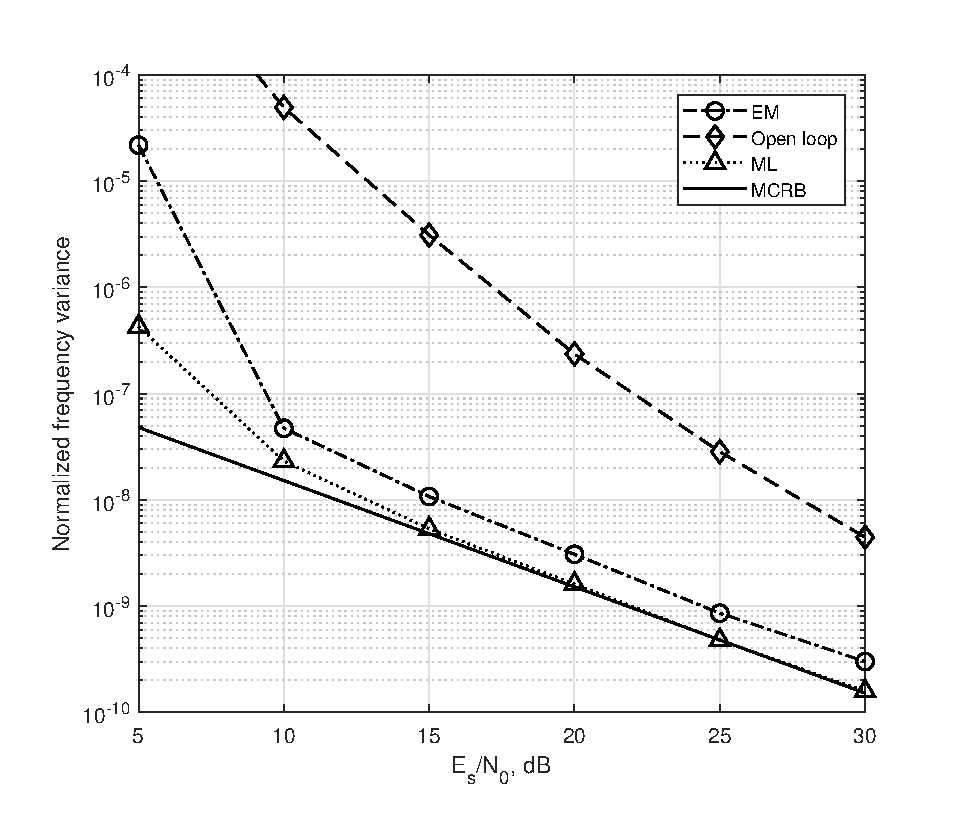
\includegraphics[width=3.1 in]{pic/per_freq-k.eps}
\caption{Performance of three carrier frequency recovery algorithms.}
\label{fig:per_freq} 
\end{figure} 
% MCRB_freq_revisit2.m

In Fig.~\ref{fig:per_freq}, the EM algorithm shows much smaller frequency variance than the open loop algorithm. 
This demonstrates its robustness for CFO estimation.
However, the performance of the classic ML algorithm is mostly the same as the MCRB, making it slightly better than the EM algorithm.
% When \(E_s/N_0\) is less than 10 dB, frequency variances of both the EM and ML algorithms grow 
It is not surprising that the classic ML algorithm provides a smaller variance than the EM algorithm in AWGN, since theoretically it is the optimum solution in these conditions. 
% Also, the EM algorithm is constrained on the resource available, and limited samples does degrade its performance. However, as has been shown above, in a multipath channel, the EM detector converges to a different solution than the ML algorithm, and this solution can provide a better synchronization parameter prior to an equalizer. As such, EM algorithms are more suitable for channels where high order statistics cannot be neglected.  

The CFO estimation performance for both the EM and classic ML algorithms in multipath channels has also been examined.
The random multipath channel described in~(\ref{eq:multi_path_2}) is used,
and the independent CFO is applied to each path.
The performance of the two algorithms has no significant difference in terms of BER if the same timing recovery is given.
This is because no ISI gain can be provided to the EM algorithm in contrast to its gain for the STO estimation.
The EM algorithm has an estimation variance that is slightly larger than that of the classic ML algorithm, similar to the results observed in AWGN channel.
Nonetheless, this demonstrates the usefulness of the proposed estimator as a universal timing recovery algorithm.
% The detail of this test is omitted due to tediousness and insignificance.  
%A There are several reasons why the the EM algorithm may have inferior performance in symbol timing and carrier recovery than the ML based algorithms.
% First, the EM based algorithms (not the EM criterion itself) are derived under a few assumptions and approximations, which are not always true in practice.
% The second reason is that the ML criterion is theoretically the optimum solution in AWGN channels, 
% where the system can be characterized by the 2nd order statistics.
% Its performance is supposed to reach the Cram\'er-Rao bound, therefore, the EM algorithms cannot achieve better performance.
% The EM algorithms are more suitable for channels where high order statistics cannot be neglected.
% * <x.liu@dal.ca> 2017-10-27T13:58:44.114Z:
% 
% I want to differentiate the criterion from the algorithm.
% we should talk about this section
% 
% ^.

% test with sea trial measurement data


%%%%%%%%%%%%%%%%%%%%%%%%%%%%%%%%%%%%%%%%%%%%%%%%%%
\section{Conclusion}
\label{sec:conc}
In this paper, the entropy minimization has been proposed as a synchronization criterion for wireless coherent receivers.
It is an alternative to the maximum likelihood criterion, which is the foundation of most of the standard synchronization algorithms. 
% By exploring the higher order statistics of the signal, entropy minimization is expected to have a better estimation performance, particularly in presence of multipath.  
The symbol timing and carrier frequency offset estimation are implemented by measuring the entropy of the eye diagram and the constellation diagram.
% * <x.liu@dal.ca> 2017-10-27T14:07:10.265Z:
% 
% at of the?
% 
% ^ <x.liu@dal.ca> 2018-02-23T14:15:39.903Z.
The optimum timing delay is found by searching the timing instant with minimum eye diagram entropy, while the carrier frequency offset is estimated by searching through a range of frequencies to minimize the constellation entropy.  

The histogram based entropy estimation method requires a large amount of computation.
Instead, in this paper, a customized fast entropy estimation algorithm has been proposed.
It is a modified version of the quadratic R\'enyi entropy and the kernel density estimation method is employed to estimate the probabilities.

% Several practical issues are addressed when applying the entropy minimization criterion to signal synchronization.
Implementation constraints have also been presented. 
The proposed symbol timing algorithm can overcome local minima, it is insensitive to the carrier frequency offset, and can be used to extract the timing delay without the need for a high oversampling rate.
The carrier frequency recovery algorithm uses block averaging to expand the estimation range without compromising accuracy. 

The estimation performance of the proposed timing and frequency recovery algorithms is compared with that of standard approaches by running a set of numerical simulations. 
It is shown that the entropy minimization has great potential and offers certain advantages for synchronization.
Particularly, in multipath channels, it provides on average a better bit error rate. 
The performance improvement is even more significant in communication systems with small excess bandwidth. 

% Specifically, by running BER simulations, it is found that the entropy minimization based algorithms can offer improved symbol timing results
% * <x.liu@dal.ca> 2017-10-27T14:20:13.538Z:
% 
% help me with this sentence 
% 
% ^ <x.liu@dal.ca> 2018-02-23T14:22:20.816Z.
% We also validated the algorithms with realistic data measured in a sea trial.
% Good tracking and compensating results are received in a time varying underwater acoustic channel.
\small
\bibliographystyle{IEEEbib}
\bibliography{Mendeley}


\end{document}